In order to test the ability of an agent to follow certain trajectories, we generate synthetic paths that act as a replacement for the ground truth AIS paths. However, the generated trajectories are not comparable to the real vessel paths because the synthetic ones get generated by arbitrary functions that output direction values and include sine functions to be "curvy" (hence the name "Curve" environment).
\par
For the main part, the environment uses three functions to sample ground truth trajectories. They combine curves, different speeds and individual directions and are specified as:

\begin{equation}\label{eq:curve_A}
\textcolor[RGB]{235,52,35}{curve\_A} = \sin \left( \frac{t}{4} \right) + 6\pi
\end{equation}
\begin{equation}
\textcolor[RGB]{20,1,244}{curve\_B} = \sin \left( \frac{t}{2} \right)+ \frac{3}{5}\pi
\end{equation}
\begin{equation}
\textcolor[RGB]{54,125,34}{curve\_C} = \sin \left( \frac{2}{3} t \right) - \frac{\pi}{6}
\end{equation}

\begin{figure}[H]
    \centering
    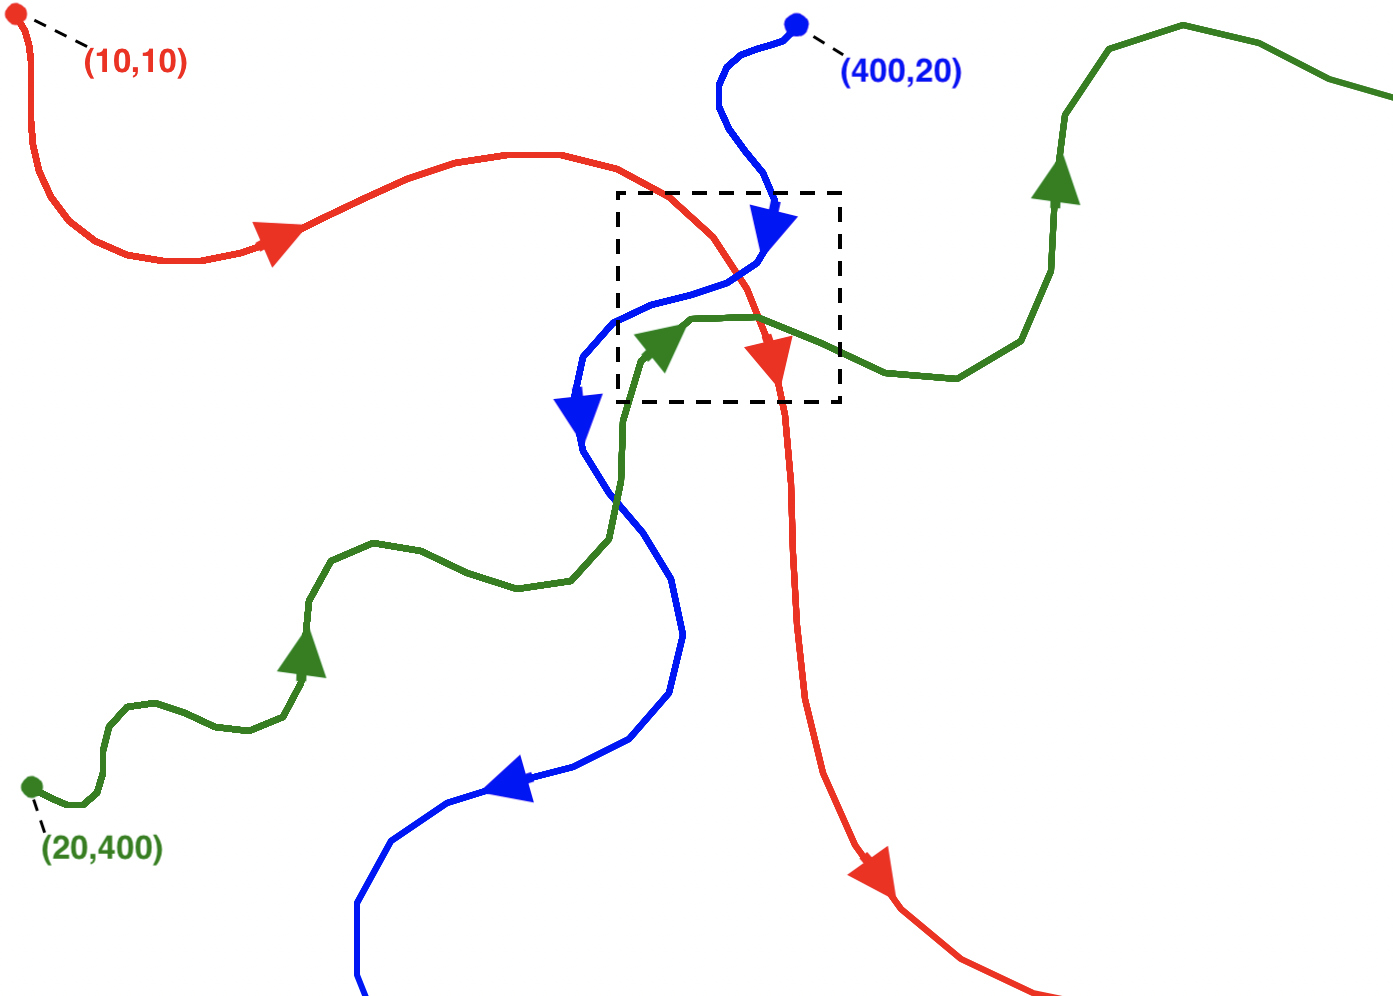
\includegraphics[width=0.75\textwidth]{images/curves.png}
    \caption{Synthetic curves with respective start positions}
    \label{fig:syntheticCurves}
\end{figure}

Generating rather complex curves instead of straight lines forces to agent to adjust its direction (and potential speed) at every timestamp. This is a test for an underlying policy to have a granular mapping from states to actions as well as the ability to recognize important (small) magnitudes of change in every state dimension. For example, we take the starting sequence of the green path generated by $curve\_C$. In a small area which translate to a small range of x and y values, the agent has to perform rapid changes to the proposed direction in order to follow the sharp turns. Additionally, as the speed of the ground truth is constantly increases, the adjustment to the direction has to slow down for consecutive timesteps as the curves get stretched and have an increased amplitude.
\par
To add to the reasons of generating paths based on those three function, the positions and directions of the resulting trajectories challenge the agent to put special emphasis on a single feature dimension - the direction.  In order to understand why this is the case, we try to see the interaction cycle (recall subchapter \ref{chap:rlframework}) from the perspective of the agent. The agent is unaware of the history of positions (the trajectory) because it just receives the latest position with potentially more information such as speed and direction (depending on the variant of the environment). As indicated by the dashed rectangle in Fig. \ref{fig:syntheticCurves}, all three curves cross the same area. If for example the agent receives a state of $\{x=400, y=250\}$, it should perform an action which represents moving towards the bottom right if the ground truth trajectory is $curve\_A$. However, the agent is unaware of the ground truth path or its type. Receiving the same or similar state in the next episode would result in the same action and choice of direction even though the internal ground truth trajectory change to $curve\_B$ and actually requires the agent to move to the bottom left. The two synthetic paths $curve\_B$ and $curve\_C$ (green and blue) take this to the extreme as they move in near opposing directions. As a result, one hypothesis is that if the state representation is purely composed of the position (x and y coordinates), the agent is unable to differentiate between the three curves, as the states belonging to the different curves are not unique.
\par
Moreover, this is a test to whether or not it is even possible to learn representations of arbitrary paths which are not all part of single family of curves and can not be classified as the same type with minor variances.
Works like the one from \cite{martinsen2018curved} concentrate on special scenarios with almost identical paths to follow while other works, for instance the one from \cite{edgardo}, split the dataset of AIS trajectories into groups of overall direction (e.g. moving from north to south or vice versa, leaving or entering the sea port, etc.). Our desired goal is more comparable to the one presented by \cite{venskus2021unsupervised} who also try to predict vessel trajectories based on AIS data but without restricting or categorizing the tracks in a major way. The only factor that they use to split the tracks is the vessel type as they found out that different vessel types generate different traffic pattern thus they use one model per vessel type \cite[p.~729]{venskus2021unsupervised}.